\begin{questions}

  \question 在粗糙的水平面上以及在光滑的水平面上分别放置相同
  的两个物体$ A $和$ B $,各施以相同的力$ F $,推行了相同的距离$ s $。两种
  情况下$ F $作的功是否相等?产生的后果是否相同?

  \question 若某力对物体不作功是否对物体运动就没有影响?

  \question 子弹水平地射入一静止放置在光滑平面上的木块阻力对
  子弹作正功还是作负功?木块所受的力对木块作正功还是作负
  功?

  \question 一个质点在几个力同时作用下的位移为$ \Delta \vec{r} = \left( 4 \vec{i} - 5 \vec{j} + 6 \vec{k} \right) $
  米,其中有一个力可表达成$ \vec{F} = \left( - 3 \vec{i} - 5 \vec{j} + 9 \vec{k} \right) $牛顿。这个力在
  这过程中作功多少?

  \question 功的数值与参考系的选择有关吗?动能的数值与参考系的
  选择有关吗?有关功能的一些关系式,如式\eqref{eqn:06.02.01}、\eqref{eqn:06.02.04}、\eqref{eqn:06.02.07}是否对任何参考系都正确?

  \question 试分别选取地面、水流为参考系来讨论下面两个问题,并
  % 189.jpg
  比较两种参考系中的结果。

  (1)一个人逆水划船,使船相对于岸静止不动,他是否作
  功?

  (2)如果他停止划船,让船顺流而下,流水对船是否作功?

  \question 试判断以下各系统的机械能是否守恒:

  (1)物体自由下落,以物体及地球作为一个系统,不计空气阻力;

  (2)物体上抛,以物体及地球作为一个系统,空气阻力不能忽略;

  (3)物体沿固定斜面下滑,以物体及地球作为一个系统,分别
  考虑有、无摩擦两种情形;

  (4)用拉力$ \vec{F} $使物体匀速上升,以物体及地球作为一个系统;

  (5)单摆的自由摆动,以摆及地球作为一个系统,不计空气阻
  力;

  (6)子弹水平地射入放在光滑水平面上的木块,以子弹及木
  块作为一个系统;

  (7)一球(或一圆盘)沿固定斜面无滑动地滚下,以物体及地
  球作为一个系统。

  \question 把一挂着的铁链对折,使它的下端和上端挂在一起。若铁
  链质量为$ m $,长为$ l $,要作多少功?

  \question 在高为的固定斜面顶上,一质量为$ m $的小物体由静止开
  \begin{figure}[h]
    \centering
    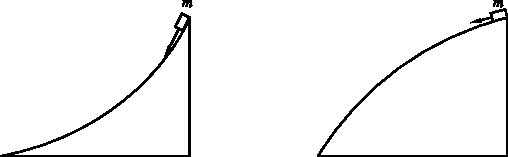
\includegraphics{figure/fig06.14}
    \caption{}
    \label{fig:06.14}
    \vspace{-0.8em}
  \end{figure}
  % 190.jpg
  \clearpage\noindent
  始下滑。求物体滑到斜面底时的速度大小若斜面是凹的或凸的
  (图\ref{fig:06.14})结果怎样?

  \question 在地面附近(可以认为$ g $是常数),以不大的初速度$ v_0 $上抛
  一个物体,不计空气阻力,问物体可上升多高?若以$ v _ { 0 } $斜抛此物,
  上升的最大高度又为多少?

  \question 若忽略地球自转,不计空气阻力,试问,逃逸速度与发
  方向有关吗?若考虑到地球的自转,人造行星应当向什么方向发
  射才比较有利?

  \question 第四章习题3中指出,飞船从地球飞向月球的途中,在通
  过地球引力区与月球引力区的分界线时,地、月对飞船的引力都
  非常小。试问,此时太阳对飞船的引力也非常小吗?如若不然,
  要注意什么问题?否则将会造成什么后果?

  \question 试解释,在荡秋千时,人怎样只依靠身体的曲伸使秋千从
  静止逐渐振荡起来。

\end{questions}
